\section{Module 2. Intensity inhomogeneity correction}
The implementation was tested with several configurations of the gaussian filter parameters and with different polynomial equations.
The first test was with the size of the filter = 170 and sigma = 20. Those parameters were set as default because they give the best results for pictures of size 256x256. In the next figures there shown results of the test which are three pictures as follows: On the left the original image, in the middle the image of bias signal and the last one is the result of dividing the original image by the inhomogeneity map.
\\
\begin{figure}[H]
\centering{}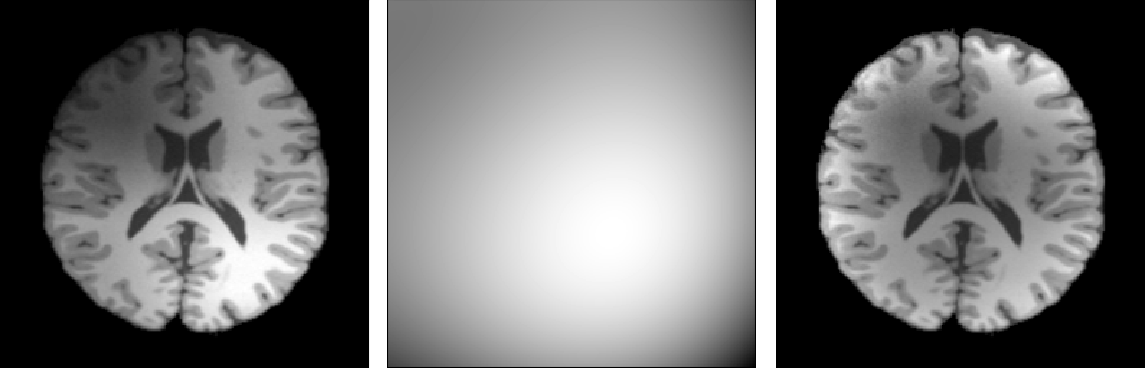
\includegraphics[scale=0.5]{figures/Module_02/test1}\caption{Original image, inhomogeneity map and the result with intensity inhomogeneity reduced. Test for filter size = 170x170, sgima = 20} 
\label{fig: test2_1}
\end{figure}
\begin{figure}[H]
\centering{}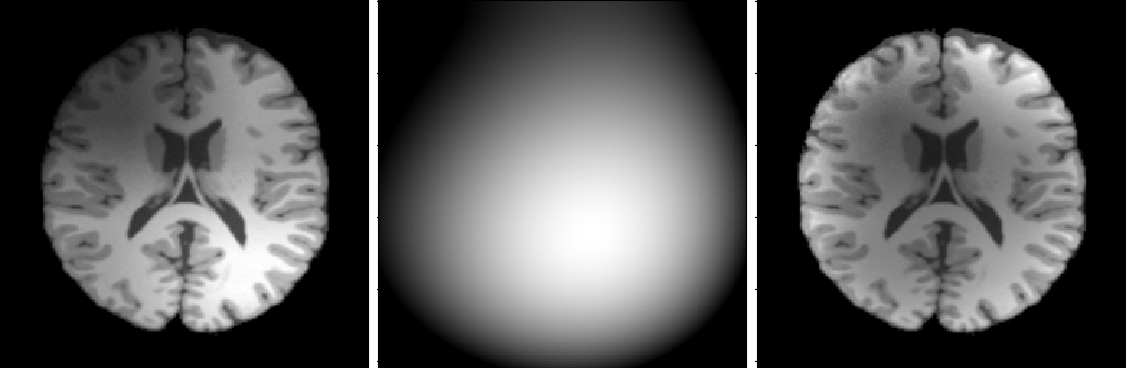
\includegraphics[scale=0.5]{figures/Module_02/test2}\caption{Original image, inhomogeneity map and the result of dividing original image by the map. Test for filter size = 170x170, sgima = 5} 
\label{fig: test2_2}
\end{figure}
\begin{figure}[H]
\centering{}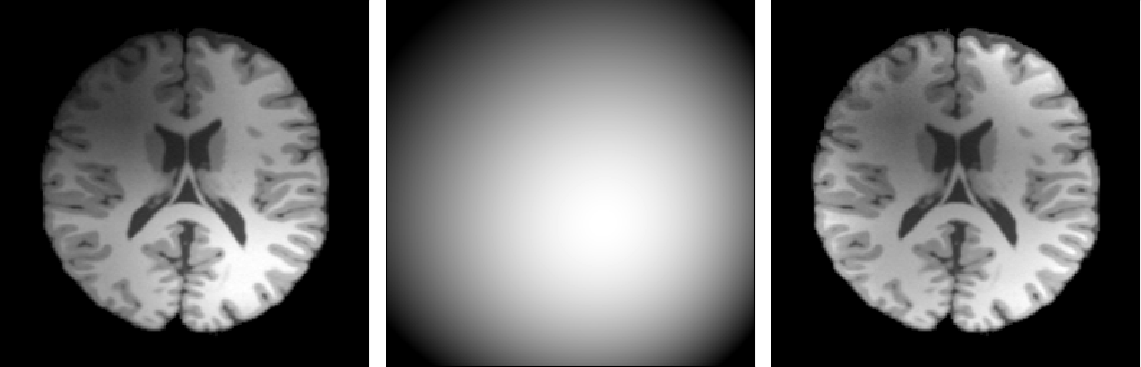
\includegraphics[scale=0.5]{figures/Module_02/test3}\caption{Original image, inhomogeneity map and the result of dividing original image by the map. Test for filter size = 170x170, sgima = 150} 
\label{fig: test2_3}
\end{figure}
\begin{figure}[H]
\centering{}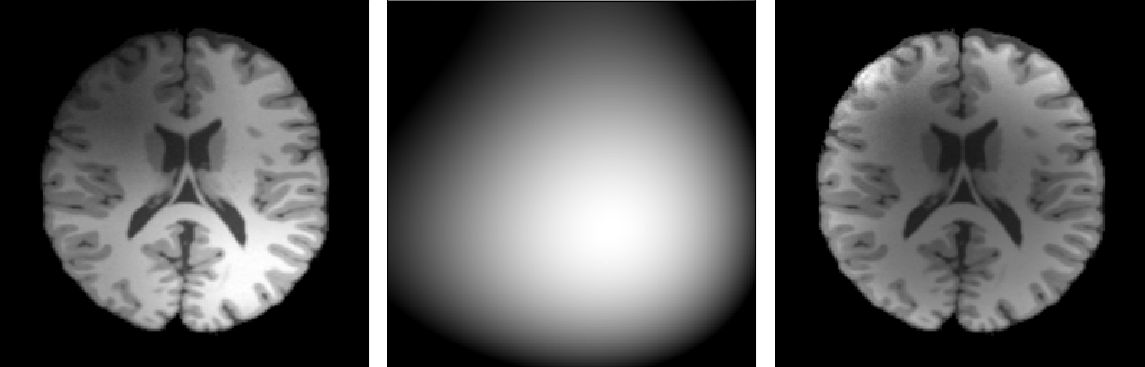
\includegraphics[scale=0.5]{figures/Module_02/test4}\caption{Original image, inhomogeneity map and the result of dividing original image by the map. Test for filter size = 20x20, sgima = 20} 
\label{fig: test2_4}
\end{figure}
There was also a test taken for an image with no inhomogeneity. The result is shown on Fig. \ref{fig: test2_5}. In conclusion, it is recommended not to use this module on images with no intensity inhomogeneity as it seems that the method could add extra inhomogeneity into a clear image.
\begin{figure}[H]
\centering{}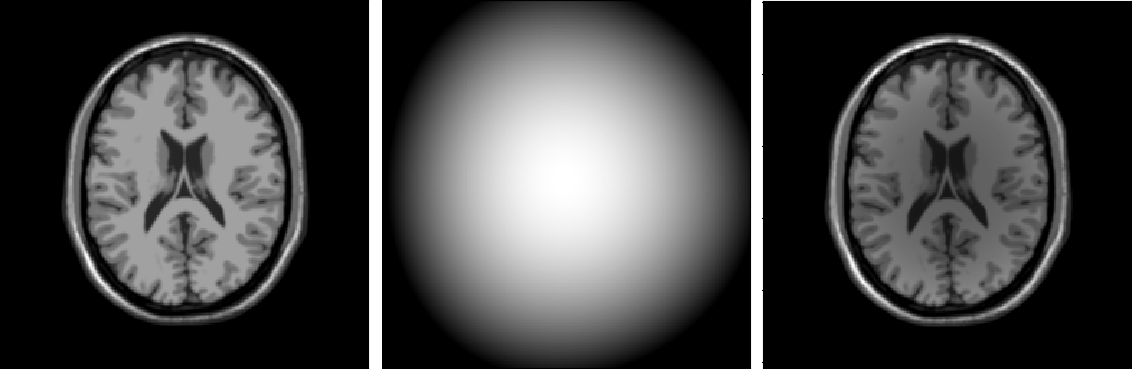
\includegraphics[scale=0.5]{figures/Module_02/test6}\caption{Original image, inhomogeneity map and the result of dividing original image by the map} 
\label{fig: test2_5}
\end{figure}
In conclusion the parameters set for the gaussian filter were chosen properly. Tests with different parameters show much worse results. This approach does not remove the inhomogeneity completely, but reduces it as much as possible. The reduction is enough to allow the next modules to receive improved data.